\documentclass[11pt,a4paper]{article}

\usepackage[table]{xcolor}
\usepackage{geometry}
\geometry{a4paper, margin=1in}
\usepackage{tcolorbox}
\usepackage{graphicx}
\usepackage{tikz}
\usetikzlibrary{shapes.geometric, arrows.meta, positioning, calc, fit, backgrounds}
\usepackage{tabularx}
\usepackage{ragged2e}
\renewcommand\tabularxcolumn[1]{>{\RaggedRight\arraybackslash}p{#1}}
\usepackage{longtable}
\usepackage{booktabs}
\usepackage{listings}
\usepackage{fancyhdr}
\usepackage{titlesec}
\usepackage{hyperref}
\usepackage{enumitem}

% --- Color Palette ---
\definecolor{navy}{HTML}{1F3A5F}
\definecolor{teal}{HTML}{0F8B8D}
\definecolor{amber}{HTML}{F2A541}
\definecolor{crimson}{HTML}{C0392B}
\definecolor{slate}{HTML}{2D3436}

\colorlet{navylight}{navy!10}
\colorlet{teallight}{teal!10}
\colorlet{amberlight}{amber!10}
\colorlet{crimsonlight}{crimson!10}
\colorlet{slatelight}{slate!10}

% --- Hyperref Setup ---
\hypersetup{
    colorlinks=true,
    linkcolor=navy,
    filecolor=teal,
    urlcolor=teal,
    pdftitle={GuardDengue: Architecture Presenter's Handbook},
}

% --- Header and Footer ---
\pagestyle{fancy}
\setlength{\headheight}{24pt}
\fancyhf{}
\fancyhead[L]{\textcolor{navy}{\textbf{GuardDengue: Presenter's Handbook}}}
\fancyfoot[C]{\textcolor{navy}{\thepage}}
\renewcommand{\headrulewidth}{0.4pt}
\renewcommand{\footrulewidth}{0.4pt}
\renewcommand{\headrule}{\hbox to\headwidth{\color{navy}\leaders\hrule height \headrulewidth\hfill}}
\renewcommand{\footrule}{\hbox to\headwidth{\color{navy}\leaders\hrule height \footrulewidth\hfill}}

% --- Titlesec Setup ---
\titleformat{\section}{\color{navy}\normalfont\Large\bfseries}{\color{navy}\thesection}{1em}{}
\titleformat{\subsection}{\color{teal}\normalfont\large\bfseries}{\color{teal}\thesubsection}{1em}{}
\titleformat{\subsubsection}{\color{slate}\normalfont\normalsize\bfseries}{\color{slate}\thesubsubsection}{1em}{}

% --- tcolorbox Environments (Native TeX Rules, Fast Compilation) ---
\tcbset{
    commonbox/.style={
        boxrule=0pt,
        leftrule=4pt,
        arc=2pt,
        fonttitle=\bfseries,
        coltitle=white,
        top=4pt,
        bottom=4pt,
        left=8pt,
        right=8pt
    }
}

\newtcolorbox{keyidea}[1][]{
    commonbox,
    colframe=navy,
    colback=navylight,
    colbacktitle=navy,
    title=Key Idea,
    #1
}

\newtcolorbox{analogy}[1][]{
    commonbox,
    colframe=teal,
    colback=teallight,
    colbacktitle=teal,
    title=Analogy,
    #1
}

\newtcolorbox{sayit}[1][]{
    commonbox,
    colframe=amber,
    colback=amberlight,
    colbacktitle=amber,
    title=Say It Script,
    #1
}

\newtcolorbox{warning}[1][]{
    commonbox,
    colframe=crimson,
    colback=crimsonlight,
    colbacktitle=crimson,
    title=Warning,
    #1
}

\newtcolorbox{qa}[1][]{
    commonbox,
    colframe=slate,
    colback=slatelight,
    colbacktitle=slate,
    title=Likely Question \& Answer,
    #1
}

% --- Listings Setup ---
\lstset{
    basicstyle=\ttfamily\small,
    backgroundcolor=\color{slatelight},
    keywordstyle=\color{navy}\bfseries,
    stringstyle=\color{teal},
    commentstyle=\color{slate}\itshape,
    showstringspaces=false,
    breaklines=true,
    frame=single,
    rulecolor=\color{slate!30},
    numbers=left,
    numberstyle=\tiny\color{slate},
    stepnumber=1,
}

% --- Custom Commands ---
\newcommand{\origintag}[2]{\textcolor{#1}{\small\textbf{[#2]}}}

\begin{document}

\begin{titlepage}
    \begin{center}
        \vspace*{2cm}
        
        
\begin{tikzpicture}
            \node[fill=navy, text=white, inner sep=15pt, rounded corners=10pt, text width=12cm, align=center] (title) {\Huge \textbf{GuardDengue: Presenter's Handbook}};
        \end{tikzpicture}
        
        \vspace{1.5cm}
        {\Large \color{teal} A Safety-Aware LLM/SLM Framework for} \\
        {\Large \color{teal} Evidence-Grounded Dengue Health Awareness}
        
        \vspace{2cm}
        {\large \color{slate} Comprehensive Walkthrough \& Defensibility Guide}
        
        \vfill
        
        
\begin{tikzpicture}
            \node[fill=teallight, text=navy, inner sep=10pt, rounded corners=5pt] (info) {
                \begin{tabular}{ll}
                    \textbf{Project:} & GuardDengue \\
                    \textbf{Review Date:} & 23 September 2026 \\
                    \textbf{Target Audience:} & Technical Presentation Evaluators
                \end{tabular}
            };
        \end{tikzpicture}
        
        \vspace{2cm}
    \end{center}
\end{titlepage}

{\color{navy}\tableofcontents}
\newpage
\section{PART I - Orientation}

\origintag{teal}{Background} Welcome to the GuardDengue Presenter's Handbook. This guide prepares you to present and defend the architecture of a safety-aware LLM/SLM framework for evidence-grounded dengue health awareness. The focus is strictly on health education, avoiding any form of diagnosis, prescribing, or autonomous triage.

\subsection{How to Use This Handbook}
\origintag{teal}{Background} Read this handbook thoroughly before your presentation. It breaks down each slide to ensure you can explain its content, understand its place in the overarching narrative, explain the deep technical logic behind the design choices, and confidently answer audience questions. Colored origin tags indicate where information originates (e.g., \origintag{navy}{Slide n}, \origintag{amber}{Review \S x}, \origintag{teal}{Background}, \origintag{slate}{Interpretation}).

\subsection{60-Second Elevator Explanation}
\begin{sayit}
\origintag{slate}{Interpretation} GuardDengue is a safety-first architecture for dengue health education. Because language models can hallucinate or blur the line between education and diagnosis, we enforce safety structurally. We separate the system into offline evidence preparation, where we strictly curate and parse medical guidelines using Docling, and an online education phase. In the online phase, LangGraph orchestrates the flow: we retrieve relevant evidence via Qdrant and a Neo4j knowledge graph, generate a response bounded strictly by that evidence, and pass it through a deterministic policy loop. If a query touches on medication safety or emergency symptoms, we completely bypass the generative model and use clinician-approved templates. This ensures we educate safely without ever diagnosing or prescribing.
\end{sayit}

\subsection{The Entire Pipeline Map}

\begin{figure}[ht]
\centering
\resizebox{\textwidth}{!}{
\begin{tikzpicture}[
    box/.style={rectangle, draw=navy, fill=navylight, rounded corners=3pt, minimum width=2.4cm, minimum height=0.9cm, align=center, font=\small},
    db/.style={cylinder, draw=teal, fill=teallight, shape border rotate=90, aspect=0.25, minimum width=2.2cm, minimum height=1.1cm, align=center, font=\small},
    arrow/.style={-{Stealth[scale=1.1]}, draw=navy, thick},
    groupbox/.style={rectangle, draw=slate!60, dashed, rounded corners=5pt, inner sep=12pt, fill=slatelight, fill opacity=0.25}
]

% --- OFFLINE EVIDENCE PREPARATION (Row y = 3.6cm) ---
\node[box] (source) at (0, 3.6) {Source Registry \\ \scriptsize (Approved Docs)};
\node[box] (docling) at (3.2, 3.6) {Module 1 \\ \scriptsize Docling Parsing};
\node[box] (chunk) at (6.4, 3.6) {Module 2 \\ \scriptsize Structure-Aware \\ \scriptsize Chunking};
\node[db] (qdrant) at (9.8, 4.4) {Qdrant \\ \scriptsize Dense + Sparse};
\node[db] (neo4j) at (9.8, 2.7) {Neo4j \\ \scriptsize Knowledge Graph};

\draw[arrow] (source) -- (docling);
\draw[arrow] (docling) -- (chunk);
\draw[arrow] (chunk.east) -- (qdrant.west);
\draw[arrow] (chunk.east) -- (neo4j.west);

\begin{scope}[on background layer]
    \node[groupbox, fit=(source) (docling) (chunk) (qdrant) (neo4j), 
          label={[text=navy, font=\bfseries\small]above:OFFLINE EVIDENCE PREPARATION}] (offline) {};
\end{scope}

% --- ONLINE EDUCATION & INFERENCE (Row y = -0.5cm) ---
\node[box] (user) at (0, -0.5) {User Request};
\node[box, fill=amberlight, draw=amber] (screen) at (3.0, -0.5) {Screening \\ \scriptsize (Emergency / Meds?)};
\node[box] (retrieval) at (6.4, -0.5) {Module 3 \\ \scriptsize Hybrid Retrieval};
\node[box] (orchestrator) at (9.8, -0.5) {Module 4 \\ \scriptsize LangGraph Orchestrator \\ \scriptsize \& Generation};
\node[box, fill=teallight, draw=teal] (verify) at (13.4, -0.5) {Verification \\ \scriptsize Gate};
\node[box] (release) at (16.6, -0.5) {Verified \\ \scriptsize Output};
\node[box, fill=crimsonlight, draw=crimson] (fallback) at (13.4, -2.4) {Safe \\ \scriptsize Fallback};

\draw[arrow] (user) -- (screen);
\draw[arrow] (screen) -- node[above, font=\scriptsize] {Education} (retrieval);
\draw[arrow] (retrieval) -- (orchestrator);
\draw[arrow] (orchestrator) -- (verify);
\draw[arrow] (verify) -- node[above, font=\scriptsize] {Pass} (release);
\draw[arrow] (verify) -- node[right, font=\scriptsize] {Fail} (fallback);
\draw[arrow] (screen.south) -- ++(0,-1.45) -- node[above, font=\scriptsize, near start] {Urgent / Meds} (fallback.west);

% Connect Dual DBs to Hybrid Retrieval (clean curved bypass)
\draw[arrow, dashed, draw=teal] (qdrant.south west) to[out=210, in=75] (retrieval.north);
\draw[arrow, dashed, draw=teal] (neo4j.south west) to[out=230, in=45] (retrieval.north east);

\begin{scope}[on background layer]
    \node[groupbox, fit=(user) (screen) (retrieval) (orchestrator) (verify) (release) (fallback), 
          label={[text=navy, font=\bfseries\small]above:ONLINE EDUCATION \& INFERENCE}] (online) {};
\end{scope}

\end{tikzpicture}
}
\caption{\origintag{slate}{Interpretation} End-to-End GuardDengue Pipeline incorporating the four modules.}
\end{figure}

\subsection{Numbering Table (Slide Map)}
\origintag{teal}{Background} Slides are numbered from zero.

\begin{table}[ht]
\centering
\rowcolors{2}{slatelight}{white}
\begin{tabular}{lll}
\toprule
\textbf{Slide Index} & \textbf{Deck Position} & \textbf{Topic} \\
\midrule
Slide 0 & 1 & Title Slide \\
Slide 1 & 2 & Why the problem needs explicit safety \\
Slide 2 & 3 & Scope and boundaries \\
Slide 3 & 4 & Two-phase architecture overview \\
Slide 4 & 5 & Module 1: Document parsing \\
Slide 5 & 6 & Module 2: Evidence-unit chunking \\
Slide 6 & 7 & Module 3 (1/2): Hybrid retrieval \\
Slide 7 & 8 & Module 3 (2/2): Neo4j evidence graph \\
Slide 8 & 9 & Module 4 (1/2): Orchestration \\
Slide 9 & 10 & Module 4 (2/2): Verification checks \\
Slide 10 & 11 & Evidence contract \\
Slide 11 & 12 & Recommended technology stack \\
Slide 12 & 13 & Evaluation plan \\
Slide 13 & 14 & Literature grounding \\
Slide 14 & 15 & Limitations \\
Slide 15 & 16 & Next steps \\
Slide 16 & 17 & Questions and feedback \\
\bottomrule
\end{tabular}
\end{table}

\newpage
\section{PART II - Slide-by-slide Walkthrough (Slides 0-5)}

% ================= SLIDE 0 =================
\subsection{Slide 0: Title Slide}
\origintag{navy}{Slide 0} 
\textbf{(a) What the slide shows:} The title slide for ``GuardDengue: A Safety-Aware LLM/SLM Framework for Evidence-Grounded Dengue Health Awareness.'' It lists the university research context, team members, supervisor (Dr. Amlan Chakraborty), and mentor (Dr. Wazib Ansar). It prominently features the boundary: ``Health education --- not diagnosis, prescribing, or autonomous triage.''

\textbf{(b) Why it sits here:} It immediately establishes the project's identity, academic context, and most importantly, the strict safety perimeter.

\textbf{(c) Deep explanation:}
\begin{analogy}
\origintag{slate}{Interpretation} Think of this system like a medical librarian, not a doctor. A librarian can safely point you to a textbook about dengue, but they will never diagnose your rash or tell you which pill to take.
\end{analogy}
\origintag{slate}{Interpretation} 1. We define the domain: dengue health awareness. 2. We specify the AI approaches (LLMs/SLMs). 3. We place a hard boundary on capabilities (no triage/diagnosis).

\textbf{(d) Link to the md:} \origintag{amber}{Review Executive Recommendation}

\begin{sayit}
\origintag{slate}{Interpretation} ``Good morning. Today we present the architecture for GuardDengue. This is a university research project aimed at providing evidence-grounded dengue health education through language models. I want to draw your attention immediately to the subtitle: this system provides education only. It explicitly avoids diagnosis, prescribing, and autonomous triage, enforcing that boundary structurally.''
\end{sayit}

\begin{qa}
\origintag{slate}{Interpretation} \textbf{Q: Why limit the scope to education instead of diagnosis?} \\
\textbf{A:} Autonomous medical diagnosis by AI introduces severe patient risk and immense regulatory liability. Our goal is safe health literacy, guiding users to correct information and appropriate care without assuming the role of a physician.
\end{qa}
\textbf{(g) Transition:} \origintag{slate}{Interpretation} ``Let's look at why explicit safety controls are necessary for this problem.''

% ================= SLIDE 1 =================
\subsection{Slide 1: Why the problem needs explicit safety}
\origintag{navy}{Slide 1} 
\textbf{(a) What the slide shows:} A comparison between unrestricted generation and evidence-grounded generation. It lists risk patterns (unsupported memory, blurring education/diagnosis, missing medication qualifiers, missed escalation) and required controls (evidence-grounded answers, scope control, hallucination mitigation, medication safety, appropriate escalation). The core caveat is: ``Neither RAG, a knowledge graph, nor an LLM verifier can guarantee zero medical misinformation.''

\textbf{(b) Why it sits here:} It justifies the entire complex architecture by showing why a simple ChatGPT wrapper fails in healthcare.

\textbf{(c) Deep explanation:}
\begin{analogy}
\origintag{slate}{Interpretation} Using a standard LLM for healthcare is like letting a creative novelist write a flight manual. The text might flow well, but it invents details when unsure. We need to force the model to behave like a strict translator of approved manuals.
\end{analogy}
\origintag{slate}{Interpretation} 1. Base models hallucinate and rely on parametric memory. 2. They give generic advice that ignores specific medication contraindications (like NSAIDs in dengue). 3. Standard RAG still allows the model to improvise if retrieval fails. 4. Therefore, structural guardrails are mandatory.

\textbf{(d) Link to the md:} \origintag{amber}{Review \S1 Literature grounding, Executive recommendation}

\begin{sayit}
\origintag{slate}{Interpretation} ``If we just connect a user to an LLM, the model might rely on unsupported memory or confidently provide a diagnosis. To prevent this, GuardDengue enforces evidence-grounded generation. We implement explicit scope controls and escalation paths. Crucially, as the review notes, no single technology---not RAG, not knowledge graphs---can guarantee zero misinformation. Safety requires layered, structural constraints.''
\end{sayit}

\begin{qa}
\origintag{slate}{Interpretation} \textbf{Q: Doesn't a Knowledge Graph solve hallucinations entirely?} \\
\textbf{A:} No. As noted in the review, a graph stores assertions, but it doesn't guarantee the LLM won't ignore them or hallucinate in its generative step. It is just one layer of a defense-in-depth strategy.
\end{qa}
\textbf{(g) Transition:} \origintag{slate}{Interpretation} ``To implement these controls, we must define exact boundaries for what the system can and cannot do.''

% ================= SLIDE 2 =================
\subsection{Slide 2: Scope and boundaries}
\origintag{navy}{Slide 2}
\textbf{(a) What the slide shows:} A table contrasting ``In scope'' (education, grounded explanations, prevention, warning-sign info, conservative escalation) and ``Out of scope'' (diagnosis, personalized treatment, dosing, autonomous severity scoring, unsupported behavior). It concludes: ``A disclaimer alone does not enforce these boundaries.''

\textbf{(b) Why it sits here:} It operationalizes the safety mandate from Slide 1 into concrete system requirements.

\textbf{(c) Deep explanation:}
\begin{analogy}
\origintag{slate}{Interpretation} A ``swim at your own risk'' sign (a disclaimer) doesn't stop drowning. We need a physical fence (architectural boundaries) around the deep end (diagnosis).
\end{analogy}
\origintag{slate}{Interpretation} 1. Education empowers the user with general facts. 2. Diagnosis maps those facts to the user's specific body. 3. The architecture must block personalized mapping, even if a user explicitly requests it.

\textbf{(d) Link to the md:} \origintag{amber}{Review \S1, Executive recommendation}

\begin{sayit}
\origintag{slate}{Interpretation} ``We strictly separate what GuardDengue will do from what it won't do. We will provide evidence-grounded explanations of warning signs. We will not provide personalized dosing or severity scoring. The architectural imperative here is that simply printing a medical disclaimer is insufficient; our system's output policies must actively block diagnostic behavior.''
\end{sayit}

\begin{qa}
\origintag{slate}{Interpretation} \textbf{Q: What if a user inputs their lab results and asks if they are safe?} \\
\textbf{A:} The system is designed to reject this. As stated in our out-of-scope rules, interpreting individual lab results or declaring someone 'safe' crosses into diagnosis. It will trigger a safe fallback advising them to consult a physician.
\end{qa}
\textbf{(g) Transition:} \origintag{slate}{Interpretation} ``With our boundaries set, let's look at the high-level architecture that enforces them.''

% ================= SLIDE 3 =================
\subsection{Slide 3: Two-phase architecture overview}
\origintag{navy}{Slide 3}
\textbf{(a) What the slide shows:} The high-level split between ``Offline Evidence Preparation'' (Source acquisition $\rightarrow$ Parsing $\rightarrow$ Clinical review $\rightarrow$ Metadata $\rightarrow$ Knowledge release) and ``Online Education'' (Screening $\rightarrow$ Retrieval $\rightarrow$ Generation $\rightarrow$ Verification $\rightarrow$ Release/fallback). Note: ``Clinical validation and incident monitoring remain required.''

\textbf{(b) Why it sits here:} It provides the mental model for the rest of the presentation, mapping the four modules to these two phases.

\textbf{(c) Deep explanation:}
\begin{analogy}
\origintag{slate}{Interpretation} It's like a restaurant. The offline phase is the prep kitchen: sourcing ingredients, inspecting them, and writing the menu. The online phase is the front of house: taking orders and serving exactly what's on the menu, nothing else.
\end{analogy}
\origintag{slate}{Interpretation} By separating these, we ensure the generative model online can only ever access data that has been rigorously vetted offline.

\textbf{(d) Link to the md:} \origintag{amber}{Review Executive recommendation}

\begin{sayit}
\origintag{slate}{Interpretation} ``Our architecture fundamentally distinguishes between offline preparation and online execution. Offline, we meticulously acquire, parse, and clinically review evidence to create a versioned release. Online, user requests are screened, evidence is retrieved, and generations are verified before release. Importantly, this technical architecture does not replace the need for continuous clinical validation and incident monitoring.''
\end{sayit}

\begin{qa}
\origintag{slate}{Interpretation} \textbf{Q: Why not just let the LLM search the web live?} \\
\textbf{A:} Live web search bypasses clinical review, breaking our evidence contract. Our offline phase ensures only approved, versioned knowledge enters the retrieval index.
\end{qa}
\textbf{(g) Transition:} \origintag{slate}{Interpretation} ``Let's dive into the first step of that offline phase: parsing complex medical documents.''

% ================= SLIDE 4 =================
\subsection{Slide 4: Module 1 --- document parsing}
\origintag{navy}{Slide 4}
\textbf{(a) What the slide shows:} The ingestion pipeline using Docling to produce a canonical representation. It highlights the need to retain table grid/headers/units and diagram branch logic. It notes VLM outputs are ``extraction hypotheses.'' Caveat: ``A successful parser status is not evidence of clinical extraction accuracy.''

\textbf{(b) Why it sits here:} Details how raw PDFs become structured, review-ready objects.

\textbf{(c) Deep explanation:}
\begin{analogy}
\origintag{slate}{Interpretation} Flattening a medical table to plain text is like taking a spreadsheet and reading it left to right without noticing columns. You lose the relationships. Docling keeps the spreadsheet structure intact.
\end{analogy}
\origintag{slate}{Interpretation} 1. Standard OCR loses table headers and spans. 2. Docling retains HTML-like structure for tables. 3. For diagrams, we might use a VLM, but because VLMs hallucinate, the output is just a hypothesis needing human review.

\textbf{(d) Link to the md:} \origintag{amber}{Review \S2 Module 1}

\begin{sayit}
\origintag{slate}{Interpretation} ``For document parsing, we recommend Docling. Standard text extraction destroys clinical tables and flowcharts. Docling preserves the cell grids, headers, and units of tables. For diagrams, we can use a VLM to extract logic, but we treat that output strictly as a hypothesis requiring human review. A 200-OK response from a parser doesn't mean the medical logic is correct.''
\end{sayit}

\begin{qa}
\origintag{slate}{Interpretation} \textbf{Q: Why not just use Unstructured or LlamaParse?} \\
\textbf{A:} Docling gives us strong local control and unified `DoclingDocument` representations that keep text, tables, and provenance together, which is ideal for our offline review process.
\end{qa}
\textbf{(g) Transition:} \origintag{slate}{Interpretation} ``Once parsed, how do we cut this document up for search without losing context?''

% ================= SLIDE 5 =================
\subsection{Slide 5: Module 2 --- evidence-unit chunking}
\origintag{navy}{Slide 5}
\textbf{(a) What the slide shows:} Structure-aware chunking showing a parent section with child chunks. Each unit preserves assertion, population, conditions, negation, warnings, and source locator. It explicitly states RAPTOR is excluded from the initial safety-critical path.

\textbf{(b) Why it sits here:} Explains how to index data so retrieval doesn't pull a sentence out of context (e.g., losing a ``DO NOT'' warning).

\textbf{(c) Deep explanation:}
\begin{analogy}
\origintag{slate}{Interpretation} If a guideline says ``Do not give aspirin to children,'' a bad chunker might split it into Chunk 1: ``Do not give'' and Chunk 2: ``Aspirin to children.'' Structure-aware chunking keeps the warning locked to the medication.
\end{analogy}
\origintag{slate}{Interpretation} 1. We chunk by logical units, not token counts. 2. We use LlamaIndex nodes to maintain parent-child links so we can expand context during retrieval. 3. We avoid RAPTOR initially because abstractive summaries can hallucinate or drop negations.

\textbf{(d) Link to the md:} \origintag{amber}{Review \S3 Module 2}

\begin{sayit}
\origintag{slate}{Interpretation} ``Module 2 handles structure-aware chunking. We must chunk around evidence units, not arbitrary token lengths. Every chunk must preserve its conditions, populations, and critical negations. By linking child chunks to their parent sections, we enable bounded context expansion during retrieval. We explicitly exclude RAPTOR from the initial path because its AI-generated summaries could inadvertently drop a critical medical warning.''
\end{sayit}

\begin{qa}
\origintag{slate}{Interpretation} \textbf{Q: Why is RAPTOR excluded if it helps with cross-document queries?} \\
\textbf{A:} RAPTOR relies on abstractive summarization. A summarizer might drop a crucial negation or population exception to save space. We need exact source fidelity for safety-critical medical answers.
\end{qa}
\textbf{(g) Transition:} \origintag{slate}{Interpretation} ``With our chunks safely stored, let's look at how we retrieve them online.''
% ================= SLIDE 6 =================
\subsection{Slide 6: Module 3 (1/2) --- hybrid retrieval}
\origintag{navy}{Slide 6}
\textbf{(a) What the slide shows:} A flow diagram of dense and sparse retrieval in Qdrant, fused and reranked, producing eligible evidence. The Neo4j graph sits alongside as a separate evidence layer. Caveat: ``Strict eligibility filters do not guarantee complete retrieval recall.''

\textbf{(b) Why it sits here:} Defines the primary semantic search mechanism.

\textbf{(c) Deep explanation:}
\begin{analogy}
\origintag{slate}{Interpretation} Dense retrieval finds concepts (like ``fever medicine''), while sparse retrieval finds exact words (like ``Paracetamol''). Using both ensures we don't miss a document just because the user used a different synonym.
\end{analogy}
\origintag{slate}{Interpretation} 1. Dense (vector) search handles synonyms and concepts. 2. Sparse (BM25/lexical) handles exact medical terms. 3. Metadata filtering ensures we only search approved documents. 4. Fusion combines the scores.

\textbf{(d) Link to the md:} \origintag{amber}{Review \S4 Module 3}

\begin{sayit}
\origintag{slate}{Interpretation} ``Module 3 employs dual indexing. First, we use Qdrant for hybrid retrieval. We apply strict metadata eligibility filters, then perform both dense vector search for concepts and sparse search for exact medical terminology. We fuse and rerank these results. Importantly, while filters ensure we only retrieve approved data, they don't guarantee perfect recall---approximate search can still miss things.''
\end{sayit}

\begin{qa}
\origintag{slate}{Interpretation} \textbf{Q: Why not use Qdrant for the graph relationships as well?} \\
\textbf{A:} Qdrant is optimized for vector similarity, not traversing multi-hop logical relationships. We use Neo4j specifically because it natively represents and queries property graphs, making clinical policies explicit and inspectable.
\end{qa}
\textbf{(g) Transition:} \origintag{slate}{Interpretation} ``Let's look at that Neo4j evidence graph now.''

% ================= SLIDE 7 =================
\subsection{Slide 7: Module 3 (2/2) --- Neo4j evidence graph}
\origintag{navy}{Slide 7}
\textbf{(a) What the slide shows:} A graph diagram: `Aspirin` $\rightarrow$ `MEMBER\_OF` $\rightarrow$ `NSAIDs` $\rightarrow$ `AVOID\_IN` $\rightarrow$ `Suspected dengue`. It highlights reviewed metadata on the edges. It notes the deterministic policy layer uses code/templates and works even if the graph is down. Caveat: ``An edge stores a reviewed assertion; it does not make the assertion true by itself.''

\textbf{(b) Why it sits here:} Shows how we handle rigid medical rules (like contraindications) that shouldn't rely on fuzzy vector search.

\textbf{(c) Deep explanation:}
\begin{analogy}
\origintag{slate}{Interpretation} Vector search is like asking a librarian for books on a topic. The graph is like checking a rigid stop-light system. If the graph says ``Red light for Aspirin in Dengue,'' we stop, regardless of what the books say.
\end{analogy}
\origintag{slate}{Interpretation} 1. We model known safety rules in a graph. 2. LLM-extracted edges must be reviewed by humans before use. 3. The graph is queried via Cypher to enforce policies.

\textbf{(d) Link to the md:} \origintag{amber}{Review \S4 Module 3}

\begin{sayit}
\origintag{slate}{Interpretation} ``Alongside vector search, we use Neo4j for a curated knowledge graph. This is where we explicitly map relationships, like Aspirin being an NSAID, which must be avoided in suspected dengue. Every edge contains provenance and review status. However, the graph just stores assertions; the actual enforcement happens via versioned Python code so that our safety policy works even if the graph database goes offline.''
\end{sayit}

\begin{qa}
\origintag{slate}{Interpretation} \textbf{Q: What happens if a medicine isn't in the Neo4j graph?} \\
\textbf{A:} Absence of an edge does not establish safety. If a medicine is unknown to our graph, the deterministic policy must conservatively route the user to consult a physician, rather than assuming it is safe to use.
\end{qa}
\textbf{(g) Transition:} \origintag{slate}{Interpretation} ``How do we coordinate the vector search, the graph, and the LLM? That brings us to Module 4.''

% ================= SLIDE 8 =================
\subsection{Slide 8: Module 4 (1/2) --- orchestration and safety workflow}
\origintag{navy}{Slide 8}
\textbf{(a) What the slide shows:} A LangGraph workflow diagram starting from user message, through screening, to either fast-track urgent/medication templates, or an education retrieval loop. The education loop includes retrieval, drafting, verification, and a repair cycle. Caveat: ``No unverified draft streaming.''

\textbf{(b) Why it sits here:} This is the operational brain of the online system, showing the actual execution path of a user request.

\textbf{(c) Deep explanation:}
\begin{analogy}
\origintag{slate}{Interpretation} LangGraph acts like a strict traffic cop. If an ambulance (emergency query) approaches, it immediately routes it to the hospital (fallback templates). Routine traffic (education queries) is routed through customs (verification) before entering the city.
\end{analogy}
\origintag{slate}{Interpretation} 1. LangGraph defines states and conditional edges. 2. Emergency routing bypasses generation completely. 3. Verification happens before the user sees a single token (no streaming unverified text).

\textbf{(d) Link to the md:} \origintag{amber}{Review \S5 Module 4}

\begin{sayit}
\origintag{slate}{Interpretation} ``Module 4 uses LangGraph to orchestrate the request. First, we screen the input. If it's an urgent concern or medication question, we bypass the LLM entirely and use approved escalation templates. For educational requests, we retrieve evidence, draft a response, and then run a strict verification gate. If it fails, it gets one bounded revision attempt. Crucially, we never stream unverified draft tokens to the user.''
\end{sayit}

\begin{qa}
\origintag{slate}{Interpretation} \textbf{Q: Why limit the revision attempts to just one?} \\
\textbf{A:} Unbounded loops can cause runaway latency and high costs. If the model fails to ground its response correctly after one revision, the safest and most efficient action is to trigger a safe fallback rather than guessing again.
\end{qa}
\textbf{(g) Transition:} \origintag{slate}{Interpretation} ``What exactly happens inside that verification gate?''

% ================= SLIDE 9 =================
\subsection{Slide 9: Module 4 (2/2) --- verification checks}
\origintag{navy}{Slide 9}
\textbf{(a) What the slide shows:} A list of 8 verification checks: Evidence support, Claim mapping, Numeric fidelity, Medication safety, Diagnosis boundary, Emergency handling, Conflicts, and Output release.

\textbf{(b) Why it sits here:} Details the criteria a generated draft must pass to be deemed safe for the user.

\textbf{(c) Deep explanation:}
\begin{analogy}
\origintag{slate}{Interpretation} This is a multi-point vehicle inspection. The car (the draft response) must pass emissions (evidence support), brakes (medication safety), and alignment (numeric fidelity). If it fails any check, it doesn't go on the road.
\end{analogy}
\origintag{slate}{Interpretation} 1. We require exact structural mapping (claims linked to chunks). 2. Numbers and units must exactly match the source. 3. Output cannot contain diagnostic phrasing.

\textbf{(d) Link to the md:} \origintag{amber}{Review \S5 Required verification behavior}

\begin{sayit}
\origintag{slate}{Interpretation} ``Before release, every draft must pass these eight checks. We verify that every claim maps to an eligible source passage. We strictly check numeric fidelity---units and operators must match exactly. We verify that no diagnostic language slipped through. If the draft fails any of these criteria and cannot be easily repaired, we discard it and provide an explicit safe fallback.''
\end{sayit}

\begin{qa}
\origintag{slate}{Interpretation} \textbf{Q: How do you verify numeric fidelity? Doesn't the LLM struggle with that?} \\
\textbf{A:} We do not rely solely on an LLM's semantic similarity judgment for numbers. We compare numbers, units, and inequality signs against the canonical Docling-extracted evidence using deterministic logic where possible.
\end{qa}
\textbf{(g) Transition:} \origintag{slate}{Interpretation} ``To make these checks work, our documents must be perfectly labeled. That requires our Evidence Contract.''

% ================= SLIDE 10 =================
\subsection{Slide 10: Evidence contract}
\origintag{navy}{Slide 10}
\textbf{(a) What the slide shows:} Required metadata fields (source, date, evidence\_level, topic), supporting metadata, and the 13-topic taxonomy. Caveat: ``Topic filters must not suppress mandatory safety evidence.''

\textbf{(b) Why it sits here:} Explains the data schema that makes the rigorous filtering and verification possible.

\textbf{(c) Deep explanation:}
\begin{analogy}
\origintag{slate}{Interpretation} The evidence contract is like a passport system. Every piece of information must have a valid ID, date of birth, and stamped visa (review status) to enter the retrieval index.
\end{analogy}
\origintag{slate}{Interpretation} 1. Without strict metadata, we can't filter out unapproved sources. 2. Topics are multi-label. 3. Safety rules are exempt from topic filtering so a semantic mismatch doesn't hide a critical warning.

\textbf{(d) Link to the md:} \origintag{amber}{Review \S1 Evidence contract shared by all modules}

\begin{sayit}
\origintag{slate}{Interpretation} ``All modules rely on a shared Evidence Contract. Every chunk of evidence must have a verified source, publication date, evidence level, and topic from our 13-category taxonomy. This ensures we never serve unreviewed or outdated data. A critical rule here is that while we filter by topic for relevance, mandatory safety rules are retrieved independently so a topic misclassification never suppresses a vital warning.''
\end{sayit}

\begin{qa}
\origintag{slate}{Interpretation} \textbf{Q: What if a document has no publication date?} \\
\textbf{A:} As stated in the review, we never substitute the ingestion time. Documents with missing or ambiguous dates are quarantined for editorial resolution. They do not enter the index.
\end{qa}
\textbf{(g) Transition:} \origintag{slate}{Interpretation} ``Taking all these modules together, here is the final software stack.''

% ================= SLIDE 11 =================
\subsection{Slide 11: Recommended technology stack}
\origintag{navy}{Slide 11}
\textbf{(a) What the slide shows:} The chosen tools: Docling, LlamaIndex nodes, Qdrant, Neo4j, Python policies, LangGraph, and an evaluated SLM/LLM. It lists optional elements (NeMo Guardrails, RAPTOR) and a simpler alternative (PostgreSQL + pgvector).

\textbf{(b) Why it sits here:} Summarizes the concrete engineering decisions derived from the architectural requirements.

\textbf{(c) Deep explanation:}
\begin{analogy}
\origintag{slate}{Interpretation} This is the bill of materials. We've designed the house; these are the specific brands of bricks and pipes we recommend using to build it.
\end{analogy}
\origintag{slate}{Interpretation} 1. Docling for parsing. 2. Qdrant for vector. 3. Neo4j for graph. 4. LangGraph for orchestration. 5. If the project is small, just use Postgres for everything (relational + pgvector) to reduce ops overhead.

\textbf{(d) Link to the md:} \origintag{amber}{Review \S7 Final recommended technology stack}

\begin{sayit}
\origintag{slate}{Interpretation} ``This is our recommended stack. Docling for parsing, LlamaIndex nodes for chunking, Qdrant and Neo4j for retrieval, and LangGraph orchestrating an evaluated language model. However, we are pragmatic: if the institution already runs PostgreSQL, utilizing pgvector and relational policy tables is a perfectly sound, simpler alternative to standing up Qdrant and Neo4j for a small guideline corpus.''
\end{sayit}

\begin{qa}
\origintag{slate}{Interpretation} \textbf{Q: Why are NeMo Guardrails only 'optional'?} \\
\textbf{A:} NeMo Guardrails provides useful supplementary rails (like prompt injection detection), but its LLM-based self-checking is fallible. It does not replace our core requirement for verified evidence and deterministic Python policies.
\end{qa}
\textbf{(g) Transition:} \origintag{slate}{Interpretation} ``Once built, how do we prove it is safe?''
% ================= SLIDE 12 =================
\subsection{Slide 12: Evaluation plan}
\origintag{navy}{Slide 12}
\textbf{(a) What the slide shows:} 9 evaluation areas for release gates (Extraction, Retrieval, Grounding, Medication safety, Emergency handling, Scope control, Reliability, Accessibility, Governance). Caveat: ``Zero observed failures is not zero real-world risk.''

\textbf{(b) Why it sits here:} Asserts that architecture alone doesn't prove safety; empirical testing is mandatory before release.

\textbf{(c) Deep explanation:}
\begin{analogy}
\origintag{slate}{Interpretation} Designing a safe car on paper is different from crash-testing it. Evaluation is the crash test. We must test the brakes (medication safety) and the airbags (emergency fallback) in real conditions.
\end{analogy}
\origintag{slate}{Interpretation} 1. We don't just evaluate the LLM, we evaluate extraction, retrieval, and governance. 2. We must use a clinician-reviewed dataset, not general benchmarks. 3. We report uncertainty intervals.

\textbf{(d) Link to the md:} \origintag{amber}{Review \S6 Clinical evaluation and release requirements}

\begin{sayit}
\origintag{slate}{Interpretation} ``Architecture alone does not establish safety. Before any public release, GuardDengue must pass rigorous evaluation across these nine areas, using a clinician-curated dataset. We test extraction fidelity, retrieval recall under strict filters, and how the system handles adversarial scope-creep. Even if we observe zero failures in testing, we must report uncertainty intervals and maintain continuous monitoring.''
\end{sayit}

\begin{qa}
\origintag{slate}{Interpretation} \textbf{Q: How do you evaluate 'Scope control'?} \\
\textbf{A:} We use adversarial test cases where users try to trick the system into diagnosing them or interpreting lab results. The system passes if it successfully triggers the safe fallback in every case.
\end{qa}
\textbf{(g) Transition:} \origintag{slate}{Interpretation} ``How does our approach align with current medical AI literature?''

% ================= SLIDE 13 =================
\subsection{Slide 13: Literature grounding}
\origintag{navy}{Slide 13}
\textbf{(a) What the slide shows:} Analysis of two papers: Amugongo et al. (2025) and Basu \& Huynh (2026). It highlights what they support (modular RAG, hallucination taxonomy, KG-verification) and what they DO NOT establish (a validated GuardDengue architecture, guaranteed % improvements).

\textbf{(b) Why it sits here:} Provides the academic defense for the design while strictly avoiding overclaims about hallucination reduction figures.

\textbf{(c) Deep explanation:}
\begin{analogy}
\origintag{slate}{Interpretation} If a study shows seatbelts reduce injuries by 45\%, you can't guarantee your specific new car will have exactly 45\% fewer injuries until you test it. We use the literature to justify building seatbelts, not to promise numbers.
\end{analogy}
\origintag{slate}{Interpretation} 1. Amugongo (2025) justifies advanced modular RAG over naive RAG. 2. Basu \& Huynh (2026) provide the input/context/fact hallucination taxonomy and support KGs. 3. We absolutely must not claim their 25-45\% reduction figures apply to our untested system.

\textbf{(d) Link to the md:} \origintag{amber}{Review \S1 Literature grounding and necessary corrections}

\begin{warning}
\origintag{crimson}{Safety Rule} NEVER transfer the reduction figures quoted from these reviews (e.g., 25-45\%) to GuardDengue.
\end{warning}

\begin{sayit}
\origintag{slate}{Interpretation} ``Our design is heavily grounded in recent literature. Amugongo 2025 motivates our modular RAG approach, and Basu \& Huynh 2026 support our use of knowledge graphs and strict hallucination taxonomies. However, I want to be perfectly clear: while this literature justifies our architectural direction, we cannot and do not claim that their specific hallucination reduction percentages automatically apply to GuardDengue. We must run our own evaluations.''
\end{sayit}

\begin{qa}
\origintag{slate}{Interpretation} \textbf{Q: Why did you include CoMT in your literature review?} \\
\textbf{A:} The original Chain of Medical Thought (CoMT) research focused on radiology reports. While it supports the concept of structured medical reasoning, our verification workflow is an engineering adaptation for education, not a direct reproduction of their clinical training method.
\end{qa}
\textbf{(g) Transition:} \origintag{slate}{Interpretation} ``Recognizing what the literature does not solve brings us to our system's known limitations.''

% ================= SLIDE 14 =================
\subsection{Slide 14: Limitations}
\origintag{navy}{Slide 14}
\textbf{(a) What the slide shows:} The known failure modes: no zero-misinformation guarantee, eligibility vs recall, extraction fallibility, routing is not triage, generative risk, and governance requirements.

\textbf{(b) Why it sits here:} Demonstrates intellectual honesty and risk awareness, crucial for medical software defense.

\textbf{(c) Deep explanation:}
\begin{analogy}
\origintag{slate}{Interpretation} This is the ``side effects'' label on our architecture. It shows we understand that every technical choice has a failure mode that must be managed by human oversight.
\end{analogy}
\origintag{slate}{Interpretation} 1. Filters can cause us to miss data. 2. Docling can still misread complex tables. 3. LLM semantic routing might misclassify an emergency. 4. Therefore, human governance and small, high-quality datasets are better than massive, noisy ones.

\textbf{(d) Link to the md:} \origintag{amber}{Review Executive recommendation, \S3, \S4}

\begin{sayit}
\origintag{slate}{Interpretation} ``We must acknowledge our limitations. There is no zero-misinformation guarantee. Our strict filters might occasionally reduce recall. Docling extraction requires human review for complex diagrams. Because semantic routing relies on models, it can fail. This is why we advocate for a small, fully clinician-reviewed knowledge base over a massive, weakly curated one, and why governance is a structural pillar of safety.''
\end{sayit}

\begin{qa}
\origintag{slate}{Interpretation} \textbf{Q: If extraction and routing are fallible, is the system safe to deploy?} \\
\textbf{A:} No system is perfectly infallible. We manage this risk by enforcing deterministic pathways for known dangers (like medications) and requiring human-in-the-loop review for offline ingestion, ensuring failures result in safe fallbacks rather than unsafe advice.
\end{qa}
\textbf{(g) Transition:} \origintag{slate}{Interpretation} ``Knowing our architecture and our limits, here is our roadmap.''

% ================= SLIDE 15 =================
\subsection{Slide 15: Next steps}
\origintag{navy}{Slide 15}
\textbf{(a) What the slide shows:} A 7-step near-term roadmap: Finalize corpus, Build Docling pipeline, Establish metadata, Implement baseline retrieval, Implement deterministic policies, Build evaluation set, Benchmark SLMs.

\textbf{(b) Why it sits here:} Provides an actionable, ordered project plan focused on the baseline before adding complex extras.

\textbf{(c) Deep explanation:}
\begin{analogy}
\origintag{slate}{Interpretation} You have to pour the foundation before you paint the walls. We need the data pipeline and the safety policies working perfectly before we worry about advanced agents or visual models.
\end{analogy}
\origintag{slate}{Interpretation} 1. Data and ingestion come first. 2. Safety policies and evaluation sets must exist before model tuning. 3. Complexity (like RAPTOR) is deferred.

\textbf{(d) Link to the md:} \origintag{amber}{Review \S7 Final recommended technology stack}

\begin{sayit}
\origintag{slate}{Interpretation} ``Our immediate focus is on building a robust, reviewable baseline. We will finalize the source registry and Docling pipeline first. Only after we have established the metadata schema, baseline retrieval, and deterministic safety policies will we benchmark our SLMs against a clinician-reviewed evaluation set. Optional complexity comes later.''
\end{sayit}

\begin{qa}
\origintag{slate}{Interpretation} \textbf{Q: Why benchmark the SLMs last?} \\
\textbf{A:} An SLM's performance is meaningless if the retrieved evidence is flawed or the safety policies are absent. We must build the environment the model will operate in before we can accurately evaluate the model itself.
\end{qa}
\textbf{(g) Transition:} \origintag{slate}{Interpretation} ``Thank you. I'm happy to take your questions.''

% ================= SLIDE 16 =================
\subsection{Slide 16: Questions and feedback}
\origintag{navy}{Slide 16}
\textbf{(a) What the slide shows:} A prompt for audience feedback on Architecture, Safety scope, and Evaluation.
\textbf{(b) Why it sits here:} Concludes the presentation and structures the Q\&A.
\textbf{(c) Deep explanation:} \origintag{slate}{Interpretation} An anchor slide to keep the conversation focused on the three core pillars of the project.
\textbf{(d) Link to the md:} \origintag{amber}{Review N/A}
\textbf{(e) Say-it script:} \origintag{slate}{Interpretation} ``That concludes the architectural overview of GuardDengue. I welcome your questions and feedback on our architecture, our safety scope, or our evaluation plan.''
\textbf{(f) Likely audience questions:} See Part V for the comprehensive rehearsal questions.
\textbf{(g) Transition:} N/A.

\newpage
\section{PART III - Deep Logic from the Review}

\origintag{teal}{Background} This section equips you with the deep technical and medical rationale for each architectural decision, preparing you to defend the framework against expert scrutiny.

\subsection{Executive Recommendation}
\origintag{amber}{Review Executive recommendation}
The recommended stack relies on Docling for parsing, structure-aware LlamaIndex nodes, Qdrant for dense/sparse retrieval, Neo4j for a curated knowledge graph, and LangGraph for orchestration. 

The core philosophy separates \textbf{offline evidence preparation} (acquiring, parsing, reviewing, and publishing versioned knowledge) from \textbf{online education} (screening, retrieving, verifying, and answering). 

\begin{warning}
\origintag{crimson}{Safety Rule} Neither RAG, a knowledge graph, nor an LLM verifier can guarantee zero medical misinformation. Safety-critical content requires reducing generative freedom. Clinical validation is an ongoing deployment requirement.
\end{warning}

\subsection{\S1 Literature Grounding and Corrections}
\origintag{amber}{Review \S1}
Our design is grounded in recent healthcare LLM reviews, but we must precisely bound our claims.

\begin{table}[ht]
\centering
\begin{tabularx}{\textwidth}{lX}
\toprule
\textbf{Literature Claim} & \textbf{Architectural Interpretation} \\
\midrule
Amugongo et al. (2025) [1] & \textbf{Verified.} Supports advanced/modular RAG but does not establish our schema as mandatory. The 45\% error rate mentioned in the review concerns unsupported URLs, not a general hallucination reduction. \\
Basu and Huynh (2026) [2] & \textbf{Verified.} Describes the input/context/fact-conflicting taxonomy and CoMT. \textbf{Do NOT transfer their 25-45\% hallucination reduction figures to GuardDengue.} \\
Tables flattening & Tables must not be indiscriminately flattened; preserve cell coordinates and headers. \\
Visual flowcharts \& VLMs & VLMs are an extraction option, not a correctness guarantee. Human review is required. \\
Emergency queries & Replace blocking with immediate safety escalation. Provide guidance, not a diagnosis. \\
NSAIDs avoidance & Block recommendations to \emph{use} them in dengue. The system can explain \emph{why} to avoid them. Route existing prescriptions to a doctor. \\
WHO public domain & WHO material is accessible, but check specific licenses. It is not automatically public domain. \\
\bottomrule
\end{tabularx}
\end{table}

\subsubsection{What the Taxonomy and CoMT Support}
The Basu/Huynh taxonomy separates input-conflicting, context-conflicting, and fact-conflicting outputs. We test these separately rather than redefining them. The CoMT (Chain of Medical Thought) research [19] concerns radiology report generation; it supports structured reasoning but does not mean asking a dengue chatbot to ``think'' automatically verifies its answers.

\subsubsection{Evidence Contract}
Every chunk in the system adheres to a strict evidence contract.

\begin{table}[ht]
\centering
\begin{tabularx}{\textwidth}{lX}
\toprule
\textbf{Field} & \textbf{Required Meaning and Validation} \\
\midrule
\texttt{source} & Canonical source identifier via an approved registry. \\
\texttt{publication\_date} & Actual publication date (ISO format). Never use ingestion time. Quarantine if missing. \\
\texttt{evidence\_level} & Documented, reviewer-assigned grade. Publisher prestige is not a grade. \\
\texttt{topic} & Controlled labels from a 13-category taxonomy. \\
\bottomrule
\end{tabularx}
\end{table}

We filter on eligibility, not blindly on inferred subject matter. Safety/warning passages are exempt from topic filtering to ensure a misclassification never suppresses them.
\subsection{\S2 Module 1: Document Parsing and Multimodal Ingestion}
\origintag{amber}{Review \S2}

\textbf{The problem it solves:} Medical guidelines contain critical safety data trapped in complex PDF tables and flowcharts. Standard OCR scrambles this data, detaching warnings from medications and mixing up table columns, which creates fatal retrieval errors downstream.

\textbf{Best practice:} Preserve a canonical structured representation. Retain the cell grid, merged headers, units, and footnotes for tables. For diagrams, extract branch logic but retain the source image. A qualified human reviewer must approve high-risk clinical logic before it becomes answerable evidence.

\subsubsection{Alternatives Comparison}
\begin{table}[ht]
\centering
\begin{tabularx}{\textwidth}{lXXX}
\toprule
\textbf{Alternative} & \textbf{Advantages} & \textbf{Limitations} & \textbf{Operations} \\
\midrule
\texttt{unstructured} & Broad support, types elements, exposes HTML. & Text-splits oversized tables. Title detection fallible. & Fast for clean docs; layout detection adds time. \\
\textbf{Docling} & Unified \texttt{DoclingDocument} retains structure, images, provenance. Local execution. & OCR/inference fallible. Exports are projections. & Higher initialization cost, but supports local caching/reproducibility. \\
LlamaParse & Managed API, layout-aware Markdown/JSON handling charts. & Generative parsing can hallucinate. API limits/costs. & Service queues and network dependency. \\
\bottomrule
\end{tabularx}
\end{table}

\textbf{Why the recommendation wins and what it costs:} We recommend \textbf{Docling} with reviewed VLM assistance. It keeps structured JSON and HTML together locally, allowing rigorous human review without third-party API dependencies. It costs more local compute (model initialization) but guarantees data provenance. 

\textbf{Failure modes:} VLM outputs for diagrams are extraction hypotheses, not ground truth. A successful 200-OK parser run does not mean the clinical logic was extracted safely. The model can hallucinate a flowchart path.

\subsubsection{Code Example: Preserve Tables and Figure Crops with Docling}
\begin{lstlisting}[language=Python]
from pathlib import Path
from docling.datamodel.base_models import ConversionStatus, InputFormat
from docling.datamodel.pipeline_options import PdfPipelineOptions
from docling.document_converter import DocumentConverter, PdfFormatOption

options = PdfPipelineOptions()
options.do_ocr = True # Enable OCR for scanned PDFs
options.do_table_structure = True # Attempt to preserve table grids
options.generate_page_images = True # Keep source page images for review
options.generate_picture_images = True # Extract figure crops

converter = DocumentConverter(
    format_options={InputFormat.PDF: PdfFormatOption(pipeline_options=options)}
)
result = converter.convert(Path("approved-guideline.pdf")) # Execute conversion
if result.status != ConversionStatus.SUCCESS:
    raise RuntimeError(f"Document requires extraction review: {result.status}")

document = result.document
output = Path("extraction")
output.mkdir(exist_ok=True)
document.save_as_json(output / "document.json") # Save canonical JSON

# Export tables as HTML to retain cell spans and structure
for index, table in enumerate(document.tables):
    (output / f"table-{index}.html").write_text(
        table.export_to_html(doc=document), encoding="utf-8"
    )

# Save source crops for human review of VLM hypotheses
for index, picture in enumerate(document.pictures):
    image = picture.get_image(document)
    if image is None:
        raise RuntimeError(f"Missing source image for picture {index}")
    image.save(output / f"picture-{index}.png")
\end{lstlisting}
\origintag{slate}{Interpretation} \textbf{Line-by-line explanation:} 
Lines 1-4 import Docling components. 
Lines 6-10 configure the pipeline to aggressively preserve structure: OCR, table grids, and image extraction are explicitly enabled. 
Lines 12-16 initialize the converter and run it against the PDF. 
Lines 17-18 check the status; anything but success triggers a hard halt for manual review. 
Lines 20-23 save the entire parsed document as a canonical JSON object. 
Lines 25-29 loop through tables, explicitly exporting them to HTML (which preserves row/col spans better than Markdown). 
Lines 31-36 loop through extracted pictures, saving the raw image crops so a human reviewer can verify any VLM-generated logic against the original diagram.
\subsection{\S3 Module 2: Semantic and Structure-Aware Chunking}
\origintag{amber}{Review \S3}

\textbf{The problem it solves:} Arbitrary token chunking (e.g., splitting every 500 tokens) routinely severs a medical assertion from its critical warning or population qualifier. If retrieval returns ``give aspirin'' without the subsequent chunk ``unless dengue is suspected,'' the resulting generation is deadly.

\textbf{Best practice:} Chunk around \textbf{evidence units}. Retain document hierarchy and explicit links between a passage and its governing warnings. Never silently truncate a critical qualifier to satisfy a token budget. 

\subsubsection{Alternatives Comparison}
\begin{table}[ht]
\centering
\begin{tabularx}{\textwidth}{lXXX}
\toprule
\textbf{Alternative} & \textbf{Advantages} & \textbf{Limitations} & \textbf{Operations} \\
\midrule
Title/Markdown & Transparent boundaries; good for clean prose. & Warnings under separate headings can detach. & Low cost; ordinary retrieval latency. \\
Parent/child structure & Retains original wording. Small matches expand safely. & Expansion can reintroduce noise. & Modest indexing overhead. \\
RAPTOR & Cross-document thematic summaries. & Generated summaries may drop negations/qualifiers. & High offline cost (clustering/LLM). \\
LangChain splitters & Lightweight, composable. & Clinical atomicity needs custom logic. & Low cost. \\
\textbf{LlamaIndex nodes} & Native metadata, parent/child/adjacency links. & Parsers don't guarantee clinical safety automatically. & Inexpensive deterministically. \\
\bottomrule
\end{tabularx}
\end{table}

\textbf{Why the recommendation wins and what it costs:} We recommend \textbf{structure-aware LlamaIndex nodes} driven by Docling boundaries, completely omitting RAPTOR initially. LlamaIndex provides the exact data structure (nodes with metadata/links) needed for bounded context expansion. The cost is the engineering effort to explicitly map clinical relationships (like \texttt{governed\_by\_warning}) rather than relying on out-of-the-box splitters.

\textbf{Failure modes:} Auto-merging parent sections can exceed context windows. If the metadata parser fails, the chunk becomes ineligible for retrieval. Generative summarizers (like RAPTOR) can hallucinate and drop the word ``not''.

\subsubsection{Code Example: Parse a Reviewed Prose Section}
\begin{lstlisting}[language=Python]
import json
from datetime import date
from pathlib import Path
from llama_index.core import Document
from llama_index.core.node_parser import MarkdownNodeParser

# Load metadata from a trusted, offline-reviewed registry
metadata = json.loads(
    Path("reviewed-section.metadata.json").read_text(encoding="utf-8")
)
required = {"source", "publication_date", "evidence_level", "topic"}
if any(not metadata.get(key) for key in required):
    raise ValueError("Missing required evidence metadata")
if metadata.get("review_status") != "approved":
    raise ValueError("Unreviewed section cannot enter the answerable index")
date.fromisoformat(metadata["publication_date"]) # Validate ISO date format

# Create LlamaIndex Document with rigorous metadata attached
section = Document(
    text=Path("reviewed-prose-section.md").read_text(encoding="utf-8"),
    metadata=metadata,
)
# Parse using Markdown structure, retaining parent/child relationships
parser = MarkdownNodeParser.from_defaults(
    include_metadata=True,
    include_prev_next_rel=True,
)
nodes = parser.get_nodes_from_documents([section])
\end{lstlisting}
\origintag{slate}{Interpretation} \textbf{Line-by-line explanation:} 
Lines 1-5 import necessary JSON, date, and LlamaIndex classes. 
Lines 8-10 load the offline-reviewed metadata JSON. 
Lines 11-17 enforce the Evidence Contract: they verify that all required fields exist, that the document is explicitly marked ``approved,'' and that the date is a valid ISO string. If any check fails, ingestion stops. 
Lines 20-23 instantiate a LlamaIndex Document, fusing the raw text with the validated metadata. 
Lines 25-28 initialize the \texttt{MarkdownNodeParser}, explicitly instructing it to keep metadata and adjacent relationships (allowing us to pull the previous/next chunk if context is needed). 
Line 29 executes the parse, yielding safety-annotated nodes ready for indexing.
\subsection{\S4 Module 3: Dual Indexing and Hybrid Retrieval}
\origintag{amber}{Review \S4}

\textbf{The problem it solves:} Standard vector search misses exact terminology (e.g., specific drug names), while exact-keyword search misses semantic intent (e.g., ``fever medicine''). Neither inherently enforces safety policies.

\textbf{Best practice:} Separate the functions. Use dense retrieval for semantics, sparse retrieval for exact medical terminology, and a curated knowledge graph for absolute safety policies. Apply strict metadata eligibility filters before retrieval. 

\subsubsection{Alternatives Comparison}
\begin{table}[ht]
\centering
\begin{tabularx}{\textwidth}{lXXX}
\toprule
\textbf{Alternative} & \textbf{Advantages} & \textbf{Limitations} & \textbf{Operations} \\
\midrule
pgvector & Relational joins, SQL constraints. & Sparse/dense fusion is manual logic. & Simple if Postgres already exists. \\
\textbf{Qdrant} & Dedicated payload indexes, built-in fusion. & Highly restrictive filters can reduce recall. & Excellent for dedicated research service. \\
Milvus & High scale, multi-vector. & Complex ops overhead. & Overkill for small medical corpus. \\
\midrule
\textbf{Neo4j} & Explicit property graph, inspectable. & Edges don't make assertions true. & Adds a second database to manage. \\
Kuzu & Embedded local graph. & Upstream repo archived (Oct 2025). & Unsafe for new maintained deployments. \\
GraphRAG & Entity discovery, community summaries. & Probabilistic; cannot enforce strict policy. & High LLM cost and hallucination risk. \\
\bottomrule
\end{tabularx}
\end{table}

\textbf{Why the recommendation wins and what it costs:} We recommend \textbf{Qdrant} for vector/sparse retrieval due to its excellent payload filtering and built-in fusion. We pair this with \textbf{Neo4j} to map strict safety relationships, ignoring Kuzu (archived) and GraphRAG (probabilistic). If ops complexity is a concern, Postgres+pgvector is an acceptable simpler alternative.

\textbf{Failure modes:} Eligibility filters restrict the search space; if they are too tight, approximate search may return zero results (eligibility $\neq$ recall). Graph servers can go down, so policies must also live in local code.

\subsubsection{Code Examples}

\textbf{Example: Recommendation: Neo4j for reviewed relationships (Cypher)}
\begin{lstlisting}[language=SQL]
(Aspirin)-[:MEMBER_OF]->(NSAIDs)
(NSAIDs)-[:AVOID_IN {
    context: "suspected_dengue",
    source_chunk_id: "...",
    corpus_release: "...",
    review_status: "approved"
}]->(DengueContext)
\end{lstlisting}
\origintag{slate}{Interpretation} This explicitly models that Aspirin belongs to the NSAID class, and NSAIDs are contraindicated in dengue. The edge holds provenance.

\textbf{Example: Filtered dense/sparse retrieval with Qdrant (Python)}
\begin{lstlisting}[language=Python]
from qdrant_client import QdrantClient, models

client = QdrantClient(url="http://localhost:6333")

# Create payload index for fast filtering BEFORE vector search
for field in ("source", "review_status", "corpus_release", "topic"):
    client.create_payload_index(
        collection_name="guarddengue", field_name=field,
        field_schema=models.PayloadSchemaType.KEYWORD, wait=True,
    )

def retrieve(dense, sparse, source_ids, release):
    if not source_ids or not release:
        raise ValueError("An approved source allowlist and release are required")
    # Define the strict eligibility filter
    eligible = models.Filter(must=[
        models.FieldCondition(key="source", match=models.MatchAny(any=source_ids)),
        models.FieldCondition(key="review_status", match=models.MatchValue(value="approved")),
        models.FieldCondition(key="corpus_release", match=models.MatchValue(value=release)),
    ])
    # Execute fused query
    return client.query_points(
        collection_name="guarddengue",
        prefetch=[
            models.Prefetch(query=dense, using="dense", filter=eligible, limit=30),
            models.Prefetch(query=sparse, using="sparse", filter=eligible, limit=30),
        ],
        query=models.FusionQuery(fusion=models.Fusion.RRF),
        query_filter=eligible, limit=8, with_payload=True,
    ).points
\end{lstlisting}
\origintag{slate}{Interpretation} Lines 6-10 establish database indices to ensure fast filtering. Lines 16-20 build the `must` filter clause enforcing the Evidence Contract (approved, specific release). Lines 22-31 run two parallel sub-queries (dense and sparse) using `Prefetch`, and fuse the results using Reciprocal Rank Fusion (RRF), returning the top 8 safe chunks.

\textbf{Example: Bounded, parameterized Neo4j policy lookup (Python)}
\begin{lstlisting}[language=Python]
import os
from neo4j import GraphDatabase

with GraphDatabase.driver(
    os.environ["NEO4J_URI"],
    auth=(os.environ["NEO4J_USER"], os.environ["NEO4J_PASSWORD"]),
) as driver:
    records, _, _ = driver.execute_query(
        """
        MATCH (d:Drug {id: $drug_id})-[:MEMBER_OF]->(c:DrugClass)
        MATCH (c)-[r:AVOID_IN]->(:ClinicalContext {id: $context})
        WHERE r.review_status = 'approved'
          AND r.corpus_release = $release
        RETURN c.id AS drug_class, r.source_chunk_id AS evidence
        """,
        drug_id="aspirin", context="suspected_dengue",
        release=os.environ["GUARDDENGUE_CORPUS_RELEASE"],
        database_="neo4j", routing_="r",
    )
\end{lstlisting}
\origintag{slate}{Interpretation} Connects securely to Neo4j. The parameterized Cypher query (lines 10-15) prevents injection. It traverses from the queried drug to its class, checks for an \texttt{AVOID\_IN} edge for the specific context, and asserts that the rule is approved for the current corpus release.
\subsection{\S5 Module 4: Orchestration and Safety Guardrails}
\origintag{amber}{Review \S5}

\textbf{The problem it solves:} A single LLM call is a black box that might ignore evidence, invent facts, or answer an emergency query with slow, meandering advice. Unconstrained agents are dangerous in healthcare.

\textbf{Best practice:} Implement a bounded, auditable workflow. Store structured outputs for verification. Separate screening, retrieval, and verification into discrete states. Never stream unverified drafts.

\subsubsection{Alternatives Comparison}
\begin{table}[ht]
\centering
\begin{tabularx}{\textwidth}{lXXX}
\toprule
\textbf{Alternative} & \textbf{Advantages} & \textbf{Limitations} & \textbf{Operations} \\
\midrule
\textbf{LangGraph} & Explicit state, DAG enforcement, controlled handoffs. & Orchestrates policy but doesn't supply the medical logic itself. & Overhead secondary to model calls; predictable. \\
LlamaIndex Workflows & Event-driven, async steps. & Dynamic dispatch can be harder to audit for safety invariants. & Good if entirely in LlamaIndex ecosystem. \\
NeMo Guardrails & Pre-built rails for input/output. & Generic models don't detect dengue nuance. Self-checks fallible. & Adds latency. Use selectively. \\
\bottomrule
\end{tabularx}
\end{table}

\textbf{Why the recommendation wins and what it costs:} We recommend \textbf{LangGraph} for its explicit, strict DAG state management. It forces the system to follow the rules (screen $\rightarrow$ retrieve $\rightarrow$ draft $\rightarrow$ verify). We recommend pure Python for the deterministic safety policies rather than relying on NeMo's probabilistic rails.

\textbf{Failure modes:} Unbounded cycles (infinite LLM repair loops). Streaming tokens directly to the user bypasses verification. LLM self-checking is not a validated medical safeguard. Missing an emergency flag is fatal.

\subsubsection{Code Examples}

\textbf{Example: The Online Flow (Text)}
\begin{lstlisting}[language=bash]
User message and relevant conversation context
  -> input normalization and safety screening
     -> reported/possible urgent concern: approved escalation response
     -> medication safety: reviewed policy/template pathway
     -> educational request:
          eligibility-filtered dense + sparse retrieval
          -> rerank + bounded source/qualifier expansion
          -> evidence sufficiency and conflict gate
          -> constrained draft
          -> deterministic policy + structured claim verification
             -> pass: release the exact verified output
             -> repairable grounding issue: one bounded revision
             -> reject, unresolved, timeout, or unavailable evidence:
                  explicit safe fallback
\end{lstlisting}
\origintag{slate}{Interpretation} This explicitly details the routing. Note that emergencies and medication queries never hit the generative LLM; they go straight to approved templates. 

\textbf{Example: Bounded LangGraph verification loop (Python)}
\begin{lstlisting}[language=Python]
from typing import Literal, TypedDict
from langgraph.graph import END, START, StateGraph

class State(TypedDict):
    question: str
    route: Literal["urgent", "education", "medication", "uncertain"]
    attempts: int
    evidence: list[dict]
    evidence_ok: bool
    draft: str
    verdict: Literal["pass", "revise", "reject"]
    answer: str

def build_workflow(nodes):
    graph = StateGraph(State)
    for name in ("screen", "urgent", "medication", "retrieve", "verify", "publish", "abstain"):
        graph.add_node(name, nodes[name])

    def draft(state):
        update = nodes["draft"](state)
        return {**update, "attempts": state["attempts"] + 1}

    def after_verification(state):
        if state["verdict"] == "pass":
            return "publish"
        if state["verdict"] == "revise" and state["attempts"] < 2:
            return "draft"
        return "abstain"

    graph.add_node("draft", draft)
    graph.add_edge(START, "screen")
    graph.add_conditional_edges("screen", lambda state: state["route"], {
        "urgent": "urgent", "medication": "medication",
        "education": "retrieve", "uncertain": "abstain",
    })
    graph.add_conditional_edges(
        "retrieve",
        lambda state: "draft" if state["evidence_ok"] else "abstain",
        {"draft": "draft", "abstain": "abstain"},
    )
    graph.add_edge("draft", "verify")
    graph.add_conditional_edges("verify", after_verification, {
        "publish": "publish", "draft": "draft", "abstain": "abstain"
    })
    for terminal in ("urgent", "medication", "publish", "abstain"):
        graph.add_edge(terminal, END)
    return graph.compile()
\end{lstlisting}
\origintag{slate}{Interpretation} Line 4 defines the typed state, ensuring type safety across the graph. Lines 16-17 register the core nodes (the python functions executing logic). Lines 23-28 define the critical verification gate logic: if the verdict is \texttt{pass}, go to \texttt{publish}. If it's \texttt{revise} AND attempts $< 2$, loop back to \texttt{draft} (bounding the loop). Otherwise, \texttt{abstain} (fallback). Lines 32-47 construct the DAG, strictly routing urgent and medication queries directly to terminal nodes, bypassing retrieval and drafting entirely.
\subsection{\S6 Clinical Evaluation and Release Requirements}
\origintag{amber}{Review \S6}

Before exposing GuardDengue to users, empirical evaluation is mandatory.

\begin{table}[ht]
\centering
\begin{tabularx}{\textwidth}{lX}
\toprule
\textbf{Evaluation Area} & \textbf{What to Measure} \\
\midrule
Extraction & Fidelity of critical values, units, table headers, flowchart branches. \\
Retrieval & Recall under strict filters, handling of empty sets. \\
Grounding & Claim-level source support, citation accuracy. \\
Medication safety & Unsafe recommendation rate (aliases, combinations, negations). \\
Emergency handling & Missed vs. unnecessary escalation. \\
Scope control & Detection of adversarial requests for diagnosis/dosing. \\
Reliability & Outages, latency, timeout handling. \\
Accessibility & Target-language readability. \\
Governance & Ownership, incident reporting, rollback mechanisms. \\
\bottomrule
\end{tabularx}
\end{table}

\begin{sayit}
\origintag{slate}{Interpretation} ``We cannot release this system based on general LLM benchmarks. We must evaluate every layer---extraction, retrieval, and grounding---against a clinician-reviewed dataset. We must deliberately test adversarial cases where users demand a diagnosis, ensuring our scope control holds up. Even if we score perfectly in tests, we must report uncertainty intervals, because zero test failures does not equal zero real-world risk.''
\end{sayit}


\subsection{\S7 Final Recommended Technology Stack}
\origintag{amber}{Review \S7}

\begin{table}[ht]
\centering
\rowcolors{2}{slatelight}{white}
\begin{tabular}{lll}
\toprule
\textbf{Layer} & \textbf{Recommendation} & \textbf{Reason} \\
\midrule
Governance & Approved source registry & Traces eligible evidence. \\
Parsing & \textbf{Docling} & Preserves rich document structure. \\
Table Storage & Canonical HTML & Keeps attributes Markdown loses. \\
Diagrams & VLM + Human review & Preserves branch logic safely. \\
Chunking & \textbf{LlamaIndex nodes} & Prevents summarization loss. \\
Retrieval & \textbf{Qdrant} dense + sparse & Direct filtered hybrid support. \\
Knowledge Graph & \textbf{Neo4j} & Inspectable clinical relationships. \\
Runtime Policies & Python rules \& templates & Reliable deterministic safety. \\
Orchestration & \textbf{LangGraph} & Explicit bounded routing. \\
Generation & Evaluated SLM/LLM & Constrained generative quality. \\
\bottomrule
\end{tabular}
\end{table}

\textbf{Simpler deployment option:} PostgreSQL + pgvector + relational policy tables.
\textbf{Excluded initially:} RAPTOR summaries, unreviewed GraphRAG, autonomous diagnosis.

\newpage
\section{PART IV - End-to-End Pipeline Trace}

\origintag{teal}{Background} This section traces an illustrative user request through the entire system, demonstrating the offline preparation, the online safety routing, and the verification loop. 

\subsection{Illustrative Trace: ``Can I take ibuprofen for my dengue fever?''}
\origintag{slate}{Interpretation} The following traces how the system handles a high-risk medication query compared to a standard educational query. Note that clinical content here uses placeholders to strictly adhere to the source documents without inventing medical facts.

\begin{figure}[ht]
\centering
\begin{tikzpicture}[
    node distance=1cm and 1cm,
    stepbox/.style={rectangle, draw=navy, fill=navylight, rounded corners, minimum width=3cm, minimum height=0.8cm, align=center, font=\small},
    decision/.style={diamond, draw=amber, fill=amberlight, aspect=2, align=center, font=\scriptsize, inner sep=1pt},
    terminal/.style={rectangle, draw=crimson, fill=crimsonlight, rounded corners, minimum width=3cm, minimum height=0.8cm, align=center, font=\small},
    arrow/.style={-{Stealth[scale=1.2]}, draw=navy, thick}
]

\node[stepbox] (offline) {Offline Release \\ \scriptsize (Docling $\rightarrow$ Qdrant/Neo4j)};
\node[stepbox, below=of offline] (input) {User Request \\ \scriptsize ``Ibuprofen for dengue?''};
\node[decision, below=of input] (screen) {Screening};

\node[terminal, left=of screen, xshift=-1cm] (emergency) {Emergency Pathway \\ \scriptsize Deterministic Template};
\node[terminal, right=of screen, xshift=1cm] (medication) {Medication Pathway \\ \scriptsize Deterministic Template};

\node[stepbox, below=1.5cm of screen] (retrieve) {Hybrid Retrieval \\ \scriptsize (Educational Route)};
\node[stepbox, below=of retrieve] (draft) {Constrained Draft};
\node[decision, below=of draft] (verify) {Verification \\ Gate};

\node[stepbox, right=of verify, xshift=1cm] (release) {Release Verified \\ Output};
\node[terminal, left=of verify, xshift=-1cm] (fallback) {Safe Fallback \\ \scriptsize (Reject/Timeout)};

\draw[arrow] (offline) -- (input);
\draw[arrow] (input) -- (screen);
\draw[arrow] (screen) -- node[above, font=\scriptsize] {Urgent} (emergency);
\draw[arrow] (screen) -- node[above, font=\scriptsize] {Meds} (medication);
\draw[arrow] (screen) -- node[right, font=\scriptsize] {Education} (retrieve);

\draw[arrow] (retrieve) -- (draft);
\draw[arrow] (draft) -- (verify);
\draw[arrow] (verify) -- node[above, font=\scriptsize] {Pass} (release);
\draw[arrow] (verify) -- node[above, font=\scriptsize] {Fail} (fallback);
\draw[arrow] (verify) to[out=25, in=335, looseness=2] node[right, font=\scriptsize] {Revise} (draft);

\end{tikzpicture}
\caption{\origintag{amber}{Review \S5} End-to-end trace diagram highlighting the emergency and medication-safety pathways.}
\end{figure}

\subsubsection{Step 1: Offline Release}
Before the user ever asks the question, the WHO dengue fact sheet [18] was parsed by Docling. Its warning to avoid NSAIDs like ibuprofen due to bleeding risk was indexed. Neo4j explicitly mapped \texttt{(Ibuprofen)-[:MEMBER\_OF]->(NSAIDs)} and \newline\texttt{(NSAIDs)-[:AVOID\_IN]->(Suspected\_Dengue)}.

\subsubsection{Step 2: Request Screening}
The user asks: \textit{``Can I take ibuprofen for my dengue fever?''}
LangGraph receives the input. The screening node detects a medication-safety intent. 
\textbf{Crucial Action:} The system \textbf{diverts} the request to the Medication Pathway. It does \emph{not} send this to the generative LLM.

\subsubsection{Step 3: The Medication-Safety Pathway (Deterministic)}
Because medication recommendations carry severe risk, the system uses a versioned Python policy and a clinician-approved template.
It queries the Neo4j policy rules (or the fallback local code). The rule confirms ibuprofen is an NSAID, which is contraindicated.
\textbf{Output:} \textit{[clinician-approved content explaining that NSAIDs such as ibuprofen should be avoided due to bleeding risk, per WHO guidelines.]}

\subsubsection{Step 4: The Emergency Pathway (Deterministic)}
If the user instead asked, \textit{``I have severe abdominal pain and vomiting, what should I do?''} the screening node flags this as an ``Urgent Concern.''
\textbf{Crucial Action:} The system immediately triggers the Emergency Pathway. It does not wait for retrieval.
\textbf{Output:} \textit{[clinician-approved content advising immediate escalation to medical care for severe symptoms, per WHO guidelines.]}

\subsubsection{Step 5: The Educational Pathway (Retrieval \& Verification)}
If the user asked, \textit{``How does the virus spread?''}:
1. \textbf{Retrieval:} Qdrant finds dense/sparse matches under the ``Transmission'' topic.
2. \textbf{Constrained Generation:} The LLM drafts a response using \emph{only} the retrieved chunks.
3. \textbf{Verification Gate:} The system checks if every generated claim maps directly to the source chunk. It verifies no numeric hallucination occurred and that no diagnostic language was used.
4. \textbf{Release:} If it passes, the exact verified text is released. If it fails, it is revised once. If it fails again, it routes to a Safe Fallback.

\newpage
\section{PART V - Presentation Readiness}

\origintag{teal}{Background} This section provides rapid-fire defenses, a ``Do NOT claim'' list, and final checklists to ensure a flawless presentation.

\subsection{25 Hardest Rehearsal Questions}

\subsubsection{Module 1: Parsing}
\textbf{1. Q:} Why Docling instead of a simple PDF text extractor? \\
\textbf{A:} Simple extractors destroy table grids and detach footnotes. Docling preserves the cell coordinates and structural hierarchy needed for medical accuracy. \\
\textbf{2. Q:} Do you trust the VLM to read medical flowcharts? \\
\textbf{A:} No. We treat VLM output as a hypothesis. A human reviewer must approve high-risk clinical logic before it enters the evidence base. \\
\textbf{3. Q:} Why not use an API like LlamaParse? \\
\textbf{A:} We want to ensure local reproducibility and tight governance without third-party API dependencies or unpredictable version changes. \\
\textbf{4. Q:} What happens if a table is split across pages? \\
\textbf{A:} Docling attempts to preserve table structure, but this is exactly why human review of the canonical JSON/HTML artifact is mandatory.

\subsubsection{Module 2: Chunking}
\textbf{5. Q:} Why are you avoiding RAPTOR? \\
\textbf{A:} RAPTOR uses abstractive summarization. For clinical safety, we cannot risk a summarizer dropping a negation (e.g., ``do not take''). \\
\textbf{6. Q:} How do LlamaIndex nodes help? \\
\textbf{A:} They maintain explicit parent/child relationships, allowing us to find a precise match but expand to the full section to ensure no warnings are missed. \\
\textbf{7. Q:} What defines an ``evidence unit''? \\
\textbf{A:} An assertion bound tightly to its population, conditions, negations, and source locator. \\
\textbf{8. Q:} Doesn't expanding context blow up the token window? \\
\textbf{A:} Expansion is bounded to the immediate parent section, mitigating token-limit risks while ensuring safety.

\subsubsection{Module 3: Retrieval}
\textbf{9. Q:} Why use both dense and sparse retrieval? \\
\textbf{A:} Dense misses exact medical terms; sparse misses semantic intent. Hybrid retrieval (via Qdrant) fused with RRF catches both. \\
\textbf{10. Q:} Why add a Graph Database if you have Qdrant? \\
\textbf{A:} Qdrant handles fuzzy search. Neo4j handles rigid, deterministic rules (e.g., Drug A is contraindicated in Condition B). \\
\textbf{11. Q:} What if the Neo4j server goes down? \\
\textbf{A:} Our deterministic policy layer uses versioned local Python rules that run even if the graph is unavailable. \\
\textbf{12. Q:} Does metadata filtering reduce recall? \\
\textbf{A:} Yes, strict filters (eligibility $\neq$ recall) might miss data, which is why we must empirically evaluate retrieval under real filters. \\
\textbf{13. Q:} Why not use Kuzu for the graph? \\
\textbf{A:} The upstream Kuzu repository was archived. We cannot build a safety-critical system on unmaintained dependencies.

\subsubsection{Module 4: Orchestration \& Guardrails}
\textbf{14. Q:} Why LangGraph over LlamaIndex Workflows? \\
\textbf{A:} LangGraph provides explicit, strict DAG state management and controlled handoffs, making the verification loop highly auditable. \\
\textbf{15. Q:} What happens if the verification gate fails? \\
\textbf{A:} The draft gets one bounded revision attempt. If it fails again, we trigger an explicit safe fallback. \\
\textbf{16. Q:} Why only one revision attempt? \\
\textbf{A:} To prevent infinite LLM repair loops, which blow up latency and costs without guaranteeing safety. \\
\textbf{17. Q:} Do you use NeMo Guardrails? \\
\textbf{A:} Only selectively. Its LLM-based self-checking is fallible and does not replace our deterministic Python policies. \\
\textbf{18. Q:} How do you stop the system from diagnosing? \\
\textbf{A:} The verification gate checks for diagnostic language. Furthermore, any prompt mapping a user's specific symptoms to a conclusion is structurally blocked. \\
\textbf{19. Q:} How do you handle emergency queries? \\
\textbf{A:} The screening node detects them and routes immediately to an approved deterministic escalation template, bypassing retrieval and generation entirely.

\subsubsection{Evaluation \& General}
\textbf{20. Q:} Did you achieve a 45\% reduction in hallucinations? \\
\textbf{A:} No. The literature (Basu/Huynh) achieved those numbers in their studies. We use their methods but must run our own evaluations. \\
\textbf{21. Q:} How do you prove the system is safe? \\
\textbf{A:} We can't prove zero risk. We prove risk reduction through rigorous evaluation across 9 gates (extraction, grounding, scope control, etc.). \\
\textbf{22. Q:} What if the user inputs lab results? \\
\textbf{A:} The system classifies this as ``out of scope'' (diagnosis) and routes to a safe fallback advising them to consult a physician. \\
\textbf{23. Q:} Is WHO data automatically public domain? \\
\textbf{A:} No. Publicly accessible does not mean public domain. We track exact licenses in the metadata contract. \\
\textbf{24. Q:} Why not a large, web-crawled database? \\
\textbf{A:} A small, fully human-reviewed knowledge base is vastly safer than a massive, weakly curated one. \\
\textbf{25. Q:} How do you check numeric fidelity? \\
\textbf{A:} We do not rely on LLM similarity. We deterministically compare generated numbers/units against the canonical extracted evidence.

\subsection{Design Choices Table}
\begin{table}[ht]
\centering
\begin{tabularx}{\textwidth}{lXX}
\toprule
\textbf{Design Choice} & \textbf{Rejected Alternative} & \textbf{Reason for Rejection} \\
\midrule
Docling & Plain Text/Markdown OCR & Destroys table grids and detaches footnotes. \\
LlamaIndex Nodes & RAPTOR & Abstractive summaries may drop critical negations. \\
Qdrant (Hybrid) & Pure Dense Search & Misses exact medical terminology. \\
Neo4j + Python & Qdrant for rules & Vector search cannot enforce rigid clinical logic. \\
LangGraph & Unconstrained Agent & Agents can ignore evidence; DAG forces a strict verification gate. \\
\bottomrule
\end{tabularx}
\end{table}

\subsection{``Do NOT Claim'' List}
\begin{warning}
\origintag{crimson}{Safety Rule} If you say these, you fail the defense.
\begin{itemize}[noitemsep]
    \item \textbf{DO NOT CLAIM} the system provides medical advice or diagnosis.
    \item \textbf{DO NOT CLAIM} RAG guarantees zero hallucinations.
    \item \textbf{DO NOT CLAIM} a 25\%-45\% hallucination reduction (these are literature figures, not our tested figures).
    \item \textbf{DO NOT CLAIM} the system will definitely stop all emergency cases perfectly (routing is model-based and fallible).
\end{itemize}
\end{warning}

\subsection{Final Checklist}
\begin{itemize}[noitemsep]
    \item [ ] I can explain the difference between education and diagnosis.
    \item [ ] I can articulate why Docling is used over standard OCR.
    \item [ ] I can explain why RAPTOR is excluded.
    \item [ ] I understand the difference between Qdrant (vectors) and Neo4j (rigid rules).
    \item [ ] I can trace the LangGraph workflow from start to verification.
    \item [ ] I know the 8 verification checks by heart.
\end{itemize}

\subsection{Glossary}
\begin{itemize}[noitemsep]
    \item \textbf{CoMT:} Chain of Medical Thought. A reasoning technique from literature.
    \item \textbf{Dense Retrieval:} Searching by semantic meaning (vectors).
    \item \textbf{Sparse Retrieval:} Searching by exact keywords (BM25).
    \item \textbf{RRF:} Reciprocal Rank Fusion. Combining dense and sparse scores.
    \item \textbf{DAG:} Directed Acyclic Graph. The rigid structure LangGraph uses to route tasks.
\end{itemize}

\subsection{References}
\origintag{amber}{Review References}
\begin{enumerate}[label={[\arabic*]}, font=\small, itemsep=2pt, parsep=0pt]
\scriptsize
\item Amugongo LM, Mascheroni P, Brooks S, Doering S, Seidel J. \textit{Retrieval augmented generation for large language models in healthcare: A systematic review.} PLOS Digital Health. 2025;4(6):e0000877.
\item Basu S, Huynh B. \textit{Mitigating hallucinations in healthcare AI: a systematic review of evidence-based strategies.} BMC Health Services Research. 2026;26:1115.
\item Unstructured: partitioning and chunking documentation.
\item Docling: document model, chunking, and export examples.
\item LlamaCloud Parse: overview and API examples.
\item LangChain: Markdown header splitting.
\item LlamaIndex: node parsers and nodes and relationships.
\item Sarthi et al. \textit{RAPTOR: Recursive Abstractive Processing for Tree-Organized Retrieval.} ICLR 2024.
\item pgvector: official repository and filtering guidance.
\item Qdrant: filtering, indexing, and hybrid queries.
\item Milvus: filtered search and multi-vector hybrid search.
\item Neo4j: Python driver documentation and Cypher manual.
\item Kuzu: archived upstream repository and README archival announcement.
\item Microsoft GraphRAG: official documentation.
\item LangGraph: workflows and agents and Graph API.
\item LlamaIndex: Workflows.
\item NVIDIA NeMo Guardrails: overview and self-check limitations.
\item WHO: Dengue fact sheets and integrated arboviral clinical-management guideline.
\item Jiang et al. Original CoMT medical report-generation research.
\item WHO: website terms of use and publishing copyright/licensing policy.
\end{enumerate}

\end{document}
